% 2009 年湖北卷文科第 6 题：三棱柱 ABC-A1B1C1。
% 来源 PDF：普通高考/2009/2009湖北文.pdf，SHA-256 f60ba7a5a2fef3449fba9474fa973c616aa52a15926b3a97f0dda6b909f4c861。
% 原页：第 1 页第 1 栏下部，书页码 525。
% 重绘依据：按原页斜视位置重绘。上底面 A1B1C1 完整可见（三条棱均为实线），
%   下底面 ABC 的 AB 被柱体遮挡，画虚线；AA1、BB1、CC1 为侧棱，CC1 由 C1 连至 C。
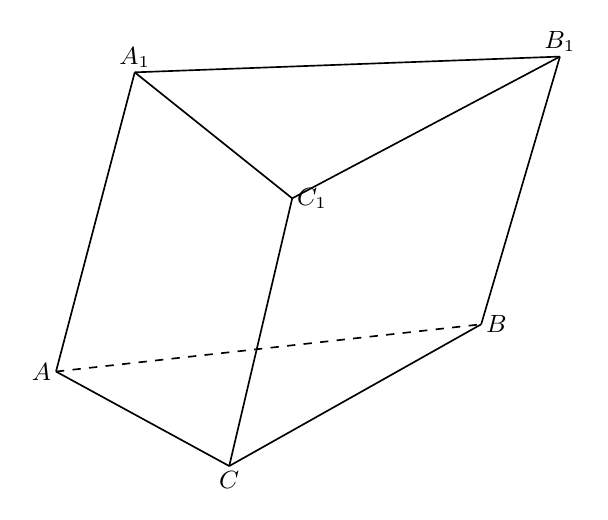
\begin{tikzpicture}[semithick, every node/.style={inner sep=1.5pt, font=\small}]
  \coordinate (A)  at (0.9,2.1);
  \coordinate (B)  at (6.3,2.7);
  \coordinate (C)  at (3.1,0.9);
  \coordinate (A1) at (1.9,5.9);
  \coordinate (B1) at (7.3,6.1);
  \coordinate (C1) at (3.9,4.3);

  % 可见棱
  \draw (A1) -- (B1);
  \draw (A1) -- (A);
  \draw (B1) -- (B);
  \draw (A1) -- (C1);
  \draw (B1) -- (C1);
  \draw (C1) -- (C);
  \draw (C) -- (A);
  \draw (C) -- (B);

  % 被遮挡的棱
  \draw[dashed] (A) -- (B);

  % 标签
  \node[above] at (A1) {$A_1$};
  \node[above] at (B1) {$B_1$};
  \node[right] at (C1) {$C_1$};
  \node[left] at (A) {$A$};
  \node[right] at (B) {$B$};
  \node[below] at (C) {$C$};
\end{tikzpicture}
